% ======================================================================
% Methods: simulation model, cavities, anchoring, active-length calibration,
% and dynamical analyses (tracking, label survival, exchange rates, wall
% Fourier, drift, flow, tilt, lobe rotation).
% Every statement checked against the solver source (mpcd/, branch `cassini`
% of niamh-overcharged), the run inputs and the analysis scripts (2026-10-05).
% Where code and RESEARCH.md disagree the code is followed and a
% "% NOTE:" comment is left. Requires \la (active length) and booktabs.
% ======================================================================

% ######################################################################
\section{Model, cavities and anchoring}
\label{sec:md-model}
% ######################################################################

\subsection{Nematic multi-particle collision dynamics with active dipoles}
\label{sec:md-mpcd}

We simulate a two-dimensional active nematic with the nematic multi-particle collision
dynamics (MPCD) solver NIAMH-MPCD
% NOTE: cite the NIAMH-MPCD method papers (nematic MPCD, Shendruk & Yeomans 2015; Hijar 2019;
% Kozhukhov et al. 2022 active MPCD; Kozhukhov, Loewe & Shendruk, Commun. Phys. 2024). User decision
% 2026-09-29: cite the method, do not re-derive it.
\cite{TODO_nematicMPCD,TODO_activeMPCD,TODO_Kozhukhov2024}.
Point particles of mass $m$ carry a velocity $\mathbf v_i$ and a unit orientation $\mathbf u_i$.
Each time step $\delta t$ consists of ballistic streaming, $\mathbf r_i\to\mathbf r_i+\mathbf v_i\delta t$
(with wall collisions, Sec.~\ref{sec:md-walls}), followed by a stochastic collision within
square cells of side $a$, whose grid is randomly shifted every step to restore Galilean
invariance (\texttt{galInv} $=1$, default). We work in MPCD units $a=m=k_BT=1$, so that the time unit is
$\tau_0=a\sqrt{m/k_BT}$; all times below are in $\tau_0$ and all lengths in cells.

\paragraph{Velocity collision.} The collision operator is NIAMH-MPCD option
\texttt{collOp}~$=21$ (\texttt{DIPOLE\_DIR\_SIG\_SUM}; routine \texttt{dipoleAndersenROT\_LC} in
\texttt{lc.c}). It is the Andersen-thermostatted, angular-momentum-conserving collision
(new velocities $\mathbf v_i'=\mathbf v_{\rm cm}+\boldsymbol\xi_i-\langle\boldsymbol\xi\rangle_c
+\dots$, with $\boldsymbol\xi_i$ drawn from the Maxwell--Boltzmann distribution at $k_BT$, plus the
angular-momentum correction, which in 2D uses the cell's moment of inertia $I_{zz}$ and also returns
to the fluid the torque exerted by the rotating nematogens) with an additional active velocity
increment. In each cell $c$ a plane is placed through the cell's centre of mass with normal equal to
the cell director $\hat{\mathbf n}_c$; every particle receives a kick
\begin{equation}
  \Delta\mathbf v_i^{\rm act}= \pm\,\delta t\;f(N_c)\,\Big(\sum_{j\in c}\frac{\zeta_j}{m_j}\Big)\,\hat{\mathbf n}_c ,
  \label{eq:md-active}
\end{equation}
with $+$ for particles on the positive side of the plane and $-$ otherwise, after which the
cell-averaged active kick is subtracted, so that momentum is conserved and the cell experiences a
force dipole along $\hat{\mathbf n}_c$ (outward kicks: extensile for $\zeta>0$). For
\texttt{collOp}~$21$ the prefactor is the \emph{sum} of the particle activities in the cell
(so the active stress grows with the cell occupancy $N_c$), modulated by the sigmoidal fall-off
\begin{equation}
  f(N_c)=\tfrac12\Big[1-\tanh\Big(\frac{N_c-\bar n(1+\sigma_p)}{\bar n\,\sigma_w}\Big)\Big],
  \label{eq:md-sigmoid}
\end{equation}
where $\bar n$ is the global mean number of particles per occupied cell (computed by
\texttt{globalDensities}) and $\sigma_w$, $\sigma_p$ are the species parameters
\texttt{sigWidth}, \texttt{sigPos}. We use the defaults $\sigma_w=\sigma_p=1$ (not set in the
inputs), so $f(\bar n)=\tfrac12[1+\tanh 1]\simeq0.88$ and the activity is suppressed in cells with
$N_c\gtrsim 2\bar n$. The factor $\delta t$ in Eq.~\eqref{eq:md-active} removes the time-step
dependence of the active forcing. (Operator $20$ uses the cell \emph{average} instead of the sum; we do
not use it.)
% NOTE: the "extensile" reading follows from the sign convention of the kick (particles on the +n side
% are pushed along +n); not separately checked against a flow-field measurement here.

\paragraph{Orientation collision.} With \texttt{lc}~$=1$ the nematic is treated with a
\emph{local} scalar order parameter $S_c$ (cell-wise eigen-decomposition of the orientation tensor).
Orientations are redrawn about $\hat{\mathbf n}_c$ from the Maier--Saupe distribution with
mean-field potential $U$ (in 2D by a Metropolis sampler, \texttt{genrand\_maierSaupeMetropolis\_2D}),
and are coupled to the flow through Jeffery-type rotation with tumbling parameter $\lambda$ and shear
susceptibility $\chi$, with rotational friction $\gamma_R$. All nematic parameters are the solver
defaults, identical to those of Ref.~\cite{TODO_Kozhukhov2024}: $U=10\,k_BT$, $\lambda=2$, $\chi=0.5$,
$\gamma_R=0.01$, $\delta t=0.1$, mean density $\bar n=20$ particles per cell.

\paragraph{Parameters.} Table~\ref{tab:md-params} lists every parameter set in, or relevant to, the
production inputs (typical inputs: \texttt{runs/cavity/server\_main/main\_act0.07/rho0.06/k06/s01},
\texttt{runs/cassini/W1\_size/H48\_ba1.6\_k06/s01}, \texttt{runs/cassini/W3\_ellipse/eps1.5\_k06/s01}).

\begin{table}[t]
\centering
\footnotesize
\caption{Simulation parameters (MPCD units $a=m=k_BT=1$). ``Default'' means the key is absent from the
input and the solver default applies (values from \texttt{read.c} and \texttt{docs/InputGuide.md}).}
\label{tab:md-params}
\begin{adjustbox}{max width=\textwidth}
\begin{tabular}{@{}p{0.25\linewidth}p{0.21\linewidth}p{0.2\linewidth}p{0.26\linewidth}@{}}
\toprule
Quantity & JSON key & Value & Remark \\
\midrule
\multicolumn{4}{@{}l}{\emph{Fluid and time stepping}}\\
time step $\delta t$ & \texttt{dt} & $0.1$ & default \\
thermal energy $k_BT$ & \texttt{kbt} & $1$ & default \\
particle mass $m$ & \texttt{mass} & $1$ & default \\
mean density $\bar n$ & \texttt{pop} & $20$ per cell & \texttt{pop} $=$ round$(20\,A_{\rm cav})$ \\
collision operator & \texttt{collOp} & $21$ & Andersen + ang.\ mom.\ + summed active dipole \\
Galilean shift / frame reset & \texttt{galInv}, \texttt{rFrame} & $1$, $1$ & defaults \\
\multicolumn{4}{@{}l}{\emph{Nematic and activity}}\\
nematic mode & \texttt{lc} & $1$ & local $S$ \\
mean-field potential $U$ & \texttt{mfpot} & $10$ & default \\
rotational friction $\gamma_R$ & \texttt{rfc} & $0.01$ & default \\
tumbling parameter $\lambda$ & \texttt{tumble} & $2$ & default \\
shear susceptibility $\chi$ & \texttt{shearSusc} & $0.5$ & default \\
activity $\zeta$ & \texttt{act} & $0.07$ & also $0$ (passive), $0.05$--$0.11$ (checks) \\
sigmoid width / position & \texttt{sigWidth}, \texttt{sigPos} & $1$, $1$ & defaults \\
\multicolumn{4}{@{}l}{\emph{Wall (one BC object)}}\\
phantom particles & \texttt{phantom} & $1$ & no-slip in cut cells \\
velocity multipliers & \texttt{MVN}, \texttt{MVT} & $-1$, $-1$ & bounce-back (no slip) \\
position shift & \texttt{DN} & $0$ & \\
orientation multipliers & \texttt{MUN}, \texttt{MUT} & $1$, $0$ & homeotropic \\
inside/outside & \texttt{inv} & $1$ & fluid inside the surface \\
surface powers & \texttt{P} & $[2,2,2,2]$ & quadric (and Cassini, see text) \\
semi-axis factors & \texttt{aInv} & $[1,1,1]$; ellipses $[\varepsilon,1,1]$ & semi-axes $R\,\texttt{aInv}_i$ \\
imposed winding $k$ & \texttt{customAnch} & $k$ ($-|k|$ mirror runs) & Sec.~\ref{sec:md-anch} \\
winding distribution & \texttt{eMode} & $0$ circles, $2$ ellipses, $3$ ovals & Sec.~\ref{sec:md-anch} \\
surface type, focal half-distance & \texttt{shape}, \texttt{cassiniA} & $1$, $a$ & ovals only, Sec.~\ref{sec:md-cassini} \\
\multicolumn{4}{@{}l}{\emph{Run length and output (in steps; $\times0.1$ for $\tau_0$)}}\\
warm-up (no output) & \texttt{warmUp} & $10^4$ & $10^3\,\tau_0$ \\
production & \texttt{simSteps} & $10^5$ & $10^4\,\tau_0$ ($4\times10^4$ steps in P1, P2, P3 high-$k$, W4) \\
defects & \texttt{defectsOut} & $20$ & $\Delta t_{\rm f}=2\,\tau_0$ \\
director field & \texttt{dirSOut} & $1000$ ($500$) & \\
flow field (interval average) & \texttt{flowOut} & $1000$ ($500$) & $100\,\tau_0$ ($50\,\tau_0$) windows\\
enstrophy field & \texttt{enstrophyOut} & $100$ & circles, seed 1 only \\
defect tracker & \texttt{defectTracker} & legacy (see text) & \texttt{tolD} $=0.01$ (default) \\
\bottomrule
\end{tabular}
\end{adjustbox}
\end{table}

\paragraph{Seeds and binaries.}
% NOTE (TODO.md): all runs made before the seed fix (l_a sweeps, R-scan, the whole server sweep
% main_act0.07 / _neg / passive) used a binary that silently ignored the input seed (xoshiro
% self-seeded from time+pid), so their "seed" values are meaningless and the runs cannot be regenerated
% bit-for-bit; they are statistically independent. Cassini/ellipse runs (office, branch binary e63155b)
% honour the seed. State this if reproducibility is claimed.
Runs of one parameter set differ only by the random seed. The circle sweep was run with a solver
build that did not honour the input seed, so its realisations are independent but not bit-wise
reproducible; all non-circular runs were made with a corrected build (branch \texttt{cassini},
commit \texttt{e63155b}), for which identical seeds give byte-identical output.

\subsection{Walls: no-slip, phantom particles and strong anchoring}
\label{sec:md-walls}

The cavity wall is a single implicit surface $W(\mathbf r)=0$ (fluid where $W<0$ after the
inversion \texttt{inv}~$=1$). For the standard shapes
$W=\sum_{i}\big[A_i(x_i-Q_i)\big]^{P_i}-R^{P_4}$ with $A_i=1/\texttt{aInv}_i$ and $P=[2,2,2,2]$,
i.e.\ an ellipse with semi-axes $R\,\texttt{aInv}_0$ (along $x$) and $R\,\texttt{aInv}_1$ (along $y$)
centred at $\mathbf Q$; circles have $\texttt{aInv}=[1,1,1]$.
A particle that crosses the wall during streaming is rewound to the crossing time, its velocity is
reversed (\texttt{MVN} $=$ \texttt{MVT} $=-1$, bounce-back), and its orientation is reset by
the anchoring rule (\texttt{oriBC}, below), using the wall normal $\mathbf n=\nabla W/|\nabla W|$ at the
collision point. With \texttt{phantom}~$=1$ every cell cut by the wall (any of its four corners outside
the fluid) is filled with phantom particles whose velocities are drawn about zero, which enforces
no-slip in partially filled cells. In the same routine (\texttt{ghostPart}, ``ghost anchoring'', enabled in
the code) the anchoring rule is applied to \emph{every} particle in a cut cell, with the normal
evaluated at the particle position, and the cell director and $S_c$ are recomputed; this
is what makes the anchoring strong.

\paragraph{Homeotropic projection.} With \texttt{MUN}~$=1$, \texttt{MUT}~$=0$ the anchoring rule
projects the particle orientation on a target axis $\hat{\mathbf e}$:
$\mathbf u\to(\mathbf u\cdot\hat{\mathbf e})\hat{\mathbf e}/|\mathbf u\cdot\hat{\mathbf e}|=\pm\hat{\mathbf e}$.
Without custom anchoring $\hat{\mathbf e}=\mathbf n$ (plain homeotropic anchoring, total charge $+1$ in a
simply connected cavity). With custom anchoring the axis $\hat{\mathbf e}$ is replaced by an imposed
axis that winds $k$ times around the wall (next section), imposing total topological charge $k$
carried by $2|k|$ half-integer defects of sign $\operatorname{sgn}k$.

\subsection{Imposed winding of the anchoring axis (\texttt{customAnch})}
\label{sec:md-anch}

When \texttt{customAnch}~$=k\neq0$, \texttt{oriBC} (\texttt{lc.c}) replaces the target axis by
$\hat{\mathbf e}=(\cos\psi_w,\sin\psi_w)$, where the imposed angle $\psi_w$ depends on the wall position
in one of four ways (\texttt{eMode}). Let $\varphi_n=\operatorname{atan2}(n_y,n_x)$ be the angle of the true
outward normal and $\varphi=\big[(\varphi_n-O_z-\pi)\bmod 2\pi\big]+\pi\in(0,2\pi]$ its value relative
to the wall orientation $O_z$ (all our walls have $O_z=0$).
\begin{description}
\item[\texttt{eMode} 0 (normal angle; circles).]
  \begin{equation}
    \psi_w=k\,\varphi+O_z .
    \label{eq:md-emode0}
  \end{equation}
  On a circle $\varphi$ is the polar angle, so the winding is uniform along the wall. On a non-circular wall the
  local imposed density follows the curvature, $\rho(s)=\frac1\pi\frac{d\psi_w}{ds}=\frac{k}{\pi}\kappa(s)$
  (tip/flank ratio $(a/b)^3$ on an ellipse with semi-axes $a>b$).
\item[\texttt{eMode} 1 (ellipse parameter).] With semi-axes $(\alpha,\beta)=(\texttt{aInv}_0,\texttt{aInv}_1)$
  (only the ratio enters) the ellipse parameter is recovered from the normal angle,
  $t=\operatorname{atan2}\!\big((\beta/\alpha)\sin\varphi,\cos\varphi\big)\bmod2\pi$, and the target axis is the
  ellipse normal at parameter $kt$: $\hat{\mathbf e}\propto\big((\beta/\alpha)\cos kt,\ \sin kt\big)$.
  % NOTE: InputGuide/RESEARCH call eMode 1 "uniform in the ellipse parameter t". It is uniform in t only on
  % average: the imposed angle is nu(kt) with tan nu = (alpha/beta) tan(kt), whose rate d nu/dt oscillates
  % with period pi/k by a factor (alpha/beta)^2 between tips and flanks of the k-fold copy. Also O_z is not
  % added back in this branch (TODO.md, harmless for O_z = 0). Not used in production runs.
\item[\texttt{eMode} 2 (arclength; ellipses).] With $t$ recovered as in mode 1,
  \begin{equation}
    \psi_w=2\pi k\,\frac{s(t)}{P}+O_z,\qquad
    s(t)=\int_0^{t}\!\sqrt{\alpha^2\sin^2t'+\beta^2\cos^2t'}\,dt',\quad P=s(2\pi),
    \label{eq:md-emode2}
  \end{equation}
  so the imposed density $\rho=2|k|/P$ is uniform along the wall. $s(t)/P$ is tabulated once per shape
  (\texttt{anchArclengthFraction}): trapezoidal integration on $8\times4096$ sub-intervals of $[0,2\pi]$,
  stored at $4097$ nodes and linearly interpolated; up to $8$ shapes are cached (keyed by $\beta/\alpha$).
  The origin $s=0$ is the $+x$ tip, where $\psi_w=0$ coincides with the normal.
\item[\texttt{eMode} 3 (arclength by polar angle; Cassini walls).] See Sec.~\ref{sec:md-cassini}.
\end{description}
On a circle all modes coincide ($s/P=\varphi/2\pi=t/2\pi$). The construction is used with integer
$k$; negative $k$ (mirror runs) imposes $2|k|$ defects of charge $-\tfrac12$.

\paragraph{Validation and resolution limit.} In passive circles ($R=15$) the anchoring is imposed with
alignment $0.96$--$0.99$, the tracker finds exactly $2|k|$ defects and net charge $k$ in $100\%$ of frames;
\texttt{customAnch} $=0$ and $1$ give identical results; $k=-2,-3$ are exact mirrors.
For an ellipse with $a=20$, $b=10$, $k=4$ (passive) the measured fraction of the director winding in
the tip regions $|x|>a/\sqrt2$ is $0.694/0.478/0.384$ for \texttt{eMode} $0/1/2$, against the predictions
$0.709/0.500/0.396$. The anchoring fails when the \emph{local} imposed spacing $1/\rho(s)$ approaches the
cell size: a resolution scan over circles (passive and active alike) gives clean anchoring for
$\rho\le0.10$, good at $0.15$, degraded at $0.20$ (alignment $\approx0.78$, up to $20\%$ of frames
missing imposed defects) and failure for $\rho\ge0.25$. We therefore restrict the analysis to
$\rho\le0.15$ (spacing $\gtrsim6.7$ cells); this is why non-circular cavities use the arclength modes,
whose local density does not grow with elongation.
% NOTE: validation numbers from RESEARCH.md (2026-09-28/29 entries; runs/cavityValidation,
% runs/emode2Validation, runs/cavity/resolution_scan); the scripts producing them were not re-run here.

\subsection{Cassini-oval walls and \texttt{eMode} 3}
\label{sec:md-cassini}

Ovals are Cassini ovals, the curves of constant product of the distances $d_{1,2}=|\mathbf r\mp a\hat{\mathbf x}|$
to two foci at $\pm a$ on the $x$ axis, implemented on the branch \texttt{cassini} of our solver repository
(\texttt{"shape": 1}, \texttt{"cassiniA"}~$=a$, $b\equiv$ \texttt{R}; \texttt{bc.c}, \texttt{mtools.c},
\texttt{lc.c}). The surface function is
\begin{equation}
  W=d_1d_2-b^2,\qquad d_{1,2}=\sqrt{(X\mp a)^2+Y^2},\quad (X,Y)=\big(A_0(x-Q_x),A_1(y-Q_y)\big),
  \label{eq:md-cassW}
\end{equation}
(sign reversed for \texttt{inv}~$=1$) rather than the textbook quartic $d_1^2d_2^2-b^4$: it describes the same
curve but scales like the circle's $r^2-R^2$ (and equals it for $a=0$), so the solver's root-finding tolerances
behave as for circles. The normal is the gradient
$\nabla(d_1d_2)=\big(A_0[\tfrac{d_2}{d_1}(X-a)+\tfrac{d_1}{d_2}(X+a)],\ A_1(\tfrac{d_2}{d_1}+\tfrac{d_1}{d_2})Y\big)$,
regular everywhere except at the foci (inside the fluid). Since no closed-form crossing time exists, wall crossings
are located with the solver's secant method (dispatched before the quadric shortcut). Setup guards enforce a fixed,
unrotated 2D wall ($\texttt{dsplc}=0$, $O=0$), no MD particles or swimmers, $0\le a<b$ (one closed wall),
and $\texttt{aInv}=[1,1,1]$ for \texttt{eMode}~3; \texttt{eMode} $1,2$ are rejected on Cassini walls. The oval
has half-length $H=\sqrt{b^2+a^2}$ and waist half-width $\sqrt{b^2-a^2}$; it is convex for $b/a\ge\sqrt2$ and has a
concave neck for $1<b/a<\sqrt2$; $a=0$ is the circle of radius $b$. For $b>a$ it is star-shaped about the centre,
with polar form
\begin{equation}
  r^2(\theta)=a^2\cos2\theta+\sqrt{b^4-a^4\sin^22\theta}.
  \label{eq:md-cass-polar}
\end{equation}

\paragraph{Anchoring (\texttt{eMode} 3).} On a concave neck the normal angle is not monotonic along the wall,
so it cannot label the wall position. Instead the polar angle of the colliding particle about the centre,
$\theta=\operatorname{atan2}(y-Q_y,x-Q_x)\bmod2\pi$, labels the wall uniquely, and
\begin{equation}
  \psi_w=2\pi k\,\frac{s(\theta)}{P},\qquad s(\theta)=\int_0^\theta\sqrt{r^2+(dr/d\theta')^2}\,d\theta' ,
  \label{eq:md-emode3}
\end{equation}
with the analytic derivative of Eq.~\eqref{eq:md-cass-polar}. $s(\theta)/P$ is tabulated per shape (keyed by
$a/b$) exactly as for \texttt{eMode}~2 (\texttt{cassiniArclengthFraction}). The particle position used is the one
after the wall collision (within one streaming step of the crossing point), which introduces an angular error of
order $|\mathbf v|\delta t/r$.
% NOTE: reports/cassini_patch_plan.md proposed r' by numerical differentiation; the code uses the analytic
% derivative (equivalent).

\paragraph{Validation.} Passive $k=3$ tests (\texttt{runs/cassini/T1}, \texttt{T2}): $a=0$ reproduces the circle of radius $15$
(alignment $0.970$/$0.961$ for \texttt{eMode} 0/3 vs $0.971$; accessible area $706.8$ vs $706.9$; charge audit $100\%$;
$6$ defects of $+\tfrac12$ per frame); $b/a=1.6$ and $1.2$ (concave) with \texttt{eMode}~3: alignment $0.976$, audit $100\%$,
accessible area within $0.1\%$ of the oval area. \texttt{eMode}~0 at $b/a=1.2$ also works (alignment $0.964$, audit $99.7\%$)
but bunches the imposed defects at the tips, whereas \texttt{eMode}~3 spreads them along the wall including the neck.
The production binary of the branch reproduces the production circle binary for a passive circle
(alignment $0.971$ vs $0.972$).

\subsection{Cavity geometries and run sets}
\label{sec:md-geom}

All cavities sit in a box of odd side lengths (smallest odd integers $\ge 2x_{\max}+2$ and $\ge2y_{\max}+2$), centred on the
central cell centre $\mathbf Q=(L_x/2,L_y/2)$. The population is fixed explicitly to $\mathrm{round}(20A)$, with $A$ the cavity area
(the solver's \texttt{dens} override would fill the whole box).

\paragraph{Circles} (\texttt{runs/cavity/gen\_cavity.py}, \texttt{gen\_sweep.py}). The control parameters are the winding $k$ and the
bare linear density of imposed defects, $\rho=2|k|/(2\pi R)$, which fixes the radius
\begin{equation}
  R=\frac{|k|}{\pi\rho},\qquad L=\lceil 2R+2\rceil_{\rm odd},\qquad N=\mathrm{round}(20\pi R^2).
\end{equation}
Parameter sets with $R<5$ are skipped. The main sweep (\texttt{server\_main/main\_act0.07}) covers
$\rho\in\{0.03,0.04,\dots,0.10,0.12,0.14,0.15,0.16,0.20,0.25,\dots,0.50\}$ and $k=1,\dots,20$, $5.1\le R\le63.7$, $\zeta=0.07$,
$3$ seeds ($834$ runs); the mirror set (\texttt{customAnch}~$=-k$) covers $\rho\le0.20$ ($570$ runs); passive references
($\zeta=0$, $10^4+3\times10^4$ steps, no flow output) exist for both ($278$ and $190$ runs, one seed). Seed~1 of every active set
writes director and flow fields every $1000$ steps and enstrophy every $100$; in this sweep all seeds wrote director and flow fields
(checked in the inputs). Only $\rho\le0.15$ is analysed (resolution limit). Example: $k=6$, $\rho=0.06$ gives $R=31.831$
($R/\la=1.43$), a $67\times67$ box and $63\,662$ particles.

\paragraph{Cassini ovals} (\texttt{runs/cassini/gen\_cassini.py}). An oval is specified by its half-length $H$ and the ratio $b/a$:
$a=H/\sqrt{1+(b/a)^2}$, $b=(b/a)\,a$. The area is computed numerically from Eq.~\eqref{eq:md-cass-polar},
$A=\tfrac12\oint r^2d\theta$ ($2\times10^4$ angles), and sets $N=\mathrm{round}(20A)$; the box uses the numerical extent of the
oval. All ovals use \texttt{eMode}~3 and the legacy defect tracker (\texttt{defectTracker}~$=0$). Run sets ($\zeta=0.07$ unless stated):
\begin{itemize}
\item P3 (size control): $H=34$ ($1.53\la$), $b/a=2.5,2.0,1.6,1.3$, $k=6$, 3 seeds, $10^4+10^5$ steps;
  high-$k$ pinched ovals $H=48$, $b/a=1.02$, $k=12,15,18,20$ (1 seed, $4\times10^4$ steps).
\item W1 (size collapse): $H=48$ ($2.16\la$), $b/a=1.3,1.6,2.0,2.5$, $k=6$, 3 seeds, $10^4+10^5$ steps.
  Example $b/a=1.6$: $a=25.44$, $b=40.70$, box $99\times67$, $N=100\,008$.
\item W2 ($k$ scan): $H=34$, $b/a=2.0,1.6$, $k=2,4,8,10,12$ (with $k=6$ from P3), 3 seeds.
\item P1/P2 (first look, 1 seed, $10^4+4\times10^4$ steps, flow every $500$ steps): $H=48$ and $64$, $b/a=1.6,1.3,1.1$;
  pinched $b/a=1.01$--$1.05$; W4 adds seeds 2--3 for $H=64$, $b/a=1.3,1.1$.
\item P4 (lobe reference): $H=30.44$, $b/a=1.8$ (area and aspect of one lobe of the $H=64$, $b/a=1.01$ oval), $k=3$, 3 seeds.
\item Passive references ($\zeta=0$): P5 ($H=34$ ovals and the W3 ellipses) and pinched-oval references in P2/P3.
\end{itemize}
The aspect ratio used to compare shapes is the ratio of the extents in $x$ and $y$ (from the wall polyline).

\paragraph{Ellipses} (\texttt{runs/cassini/gen\_ellipse.py}, set W3). At fixed area $A=2500$ and aspect $\varepsilon$:
semi-axes $\mathcal A=\sqrt{A\varepsilon/\pi}$ (along $x$), $\mathcal B=\mathcal A/\varepsilon$, implemented as
$\texttt{R}=\mathcal B$, $\texttt{aInv}=[\varepsilon,1,1]$, \texttt{eMode}~2, $N=\mathrm{round}(20\pi\mathcal A\mathcal B)=50\,000$;
the generator refuses tip radii $\mathcal B^2/\mathcal A<5$. Set W3: $\varepsilon=1.2,1.5,2.0$, $k=6$, 2 seeds, $10^4+10^5$ steps.
Example $\varepsilon=1.5$: $\mathcal A=34.55$, $\mathcal B=23.03$, box $73\times49$, tip radius $15.4$.

\paragraph{Size and density measures.} For non-circular cavities the imposed density is $\rho=2|k|/P$ with $P$ the
perimeter, and sizes are compared through $\sqrt{A/\pi}$, the half-length, the inscribed radius and $2A/P$
(all normalised by $\la$, Sec.~\ref{sec:md-la}).

\subsection{Defect detection}
\label{sec:md-defects}

Defects are found on the fly from the cell directors (output \texttt{defects.dat} every $20$ steps).
The charge of cell $(i,j)$ is the winding of the director around its eight neighbours,
$q_{ij}=\frac1{2\pi}\sum_{m=1}^{8}\delta\theta_m$, with each $\delta\theta_m$ the signed smallest angle between
consecutive neighbour directors (head--tail symmetric). Cells with $\big||q|-\tfrac12\big|<\texttt{tolD}=0.01$
are clustered into defects of the same sign; a defect's position is the mean of its cells' centres and its
charge the mean of their charges, and its orientation is the circular mean of the cell orientations
$\psi=\frac{q}{1-q}\operatorname{atan2}\!\big(\sum(\operatorname{sgn}q\,\partial_xQ_{xy}-\partial_yQ_{xx}),
\sum(\partial_xQ_{xx}+\operatorname{sgn}q\,\partial_yQ_{xy})\big)$, computed with centred differences of the
cell $Q$ tensor over the eight neighbours (period $2\pi$ for $+\tfrac12$, $2\pi/3$ for $-\tfrac12$).
All production runs used the legacy single-pass clustering (the circle sweep because the server binary predated the
union-find tracker, the oval runs explicitly with \texttt{defectTracker}~$=0$). Inside cavities the two trackers give
identical defect lists (251/251 frames tested; byte-identical output in a $k=6$, $\rho=0.06$ test).
% NOTE: gen_cassini.py's docstring says "same settings as gen_cavity.py (... legacy tracker)", but
% gen_cavity.py does not set defectTracker (production default is 1). The circle sweep ran legacy only
% because the old server binary had no tracker switch (RESEARCH 2026-10-03). Running seeds s04-s10
% (launched 2026-10-05) use the union-find tracker.

\subsection{Active-length calibration}
\label{sec:md-la}

The activity enters all results through the active length $\la$, measured in unconfined systems
(\texttt{runs/activeLength}, script \texttt{active\_length.py}) as
\begin{equation}
  \la=\sqrt{A_{\rm eff}/\langle N\rangle},
  \label{eq:md-la}
\end{equation}
with $\langle N\rangle$ the time-averaged number of defects (both signs) in the stationary state.

\paragraph{Runs.} Periodic $L\times L$ boxes (\texttt{domainWalls}~$=1$), mean density $20$, \texttt{collOp}~$21$, no warm-up,
defects every $20$ steps; $L=100$ ($3\times10^4$ steps, $\zeta=0.050$--$0.090$ in steps of $0.005$) and $L=200$
($8\times10^5$ particles, $2.5\times10^4$ steps $=2500\,\tau_0$, $\zeta=0.05,0.07,0.09$; additional $\zeta=0.06$, $0.11$ with 2 seeds).

\paragraph{Effective area.} The legacy tracker skips the outermost layer of cells (it cannot form the eight-neighbour loop
there), so $A_{\rm eff}=(L-2)^2$; the naive $L^2$ value is also recorded.

\paragraph{Transient removal.} The start of the stationary part is chosen automatically (Chodera's criterion): the start index
$t_0$ maximises the number of effectively independent samples $n_{\rm eff}(t_0)=(n-t_0)/[2\tau_{\rm int}(N_{t_0:n})]$, scanning
$t_0$ in steps of $\max(1,\lfloor n/200\rfloor)$ frames up to $n-20$.

\paragraph{Errors.} The integrated autocorrelation time is $\tau_{\rm int}=\tfrac12+\sum_{l=1}^{M}\rho_l$, with $\rho_l$ the
normalised autocorrelation of $N(t)$ (FFT) and Sokal's self-consistent window, the smallest $M$ with $M\ge5\tau_{\rm int}(M)$.
The standard error is $\sigma_N/\sqrt{n_{\rm eff}}$ with $n_{\rm eff}=n/(2\tau_{\rm int})$, cross-checked against $10$ contiguous
blocks, and propagated as $\delta\la=\tfrac12\la\,\delta N/\langle N\rangle$. Stationarity is checked by the difference of the two half
means in units of $\sqrt2\,\delta N$ ($|{\rm drift}|>2$ flags non-stationarity).

\paragraph{Counting checks.} Four estimators are compared: all frames; only charge-neutral frames ($|Q_{\rm net}|<0.25$); same-sign defects
closer than $1.5$ cells (minimum image) merged by union-find; merged and neutral. Merging changes nothing (no split defects), and the
neutral filter (which keeps only $47$--$59\%$ of frames at $L=200$ because of defects lost in the skipped edge layer) is not used. The
quoted values use all frames.

\paragraph{Result.} At $\zeta=0.07$, $L=200$: stationary from $t=108$, $\langle N\rangle=79.5\pm1.9$, $\tau_{\rm int}=25\,\tau_0$,
$n_{\rm eff}=47$, $\la=22.21\pm0.26$. $L=100$ gives $21.36\pm0.47$ ($1.6\sigma$ apart; no consistent finite-size trend over the three
activities, box$/\la=4$--$5$ vs $8$--$10$). We use $\la(0.07)=22.2\pm0.3$ throughout (\texttt{LA = 22.21} in the plotting scripts).
For the activity checks: $\la=26.16\pm0.23$ ($\zeta=0.05$), $24.33\pm0.09$ ($0.06$, 2 seeds), $20.66\pm0.12$ ($0.09$), $19.06\pm0.09$ ($0.11$,
2 seeds). Seed-to-seed differences at $\zeta=0.06$, $0.11$ are $1.2$--$1.5$ standard errors, so single-seed errors are somewhat optimistic.
% NOTE: user decision (RESEARCH, Publication plan): the paper does not report the l_a(zeta) scaling, only the calibration l_a(0.07).
% NOTE: one seed per activity at L = 200 for 0.05/0.07/0.09; pre-seed-fix binary (seeds 20001-20003 in the inputs not honoured).

\paragraph{Compressibility.} Density fluctuations and Mach numbers were measured in $100^2$ periodic boxes
(\texttt{densSDOut}~$=20$, \texttt{flowOut}~$=100$, $3000+3000$ steps, one seed): the standard deviation of the particle number per
cell rises from $6.06$ ($\zeta=0.05$) to $9.83$ ($0.09$), against the Poisson value $\sqrt{20}=4.47$; at $\zeta=0.07$ it is $8.05$, with
rms Mach number $v_{\rm rms}/c_s=0.84$ (isothermal $c_s=\sqrt{k_BT/m}=1$; the $99$th percentile is $1.67$). In cavities the circulating
flow stratifies the density radially: for $k=8$ at $R=1.43\la$, $\zeta=0.07$, the mean occupancy is $\approx25$ within $5$ cells of the
wall and $\approx14$ at the centre (more than $20$ cells from the wall). Because \texttt{collOp}~$21$ sums the activity over the cell
[Eq.~\eqref{eq:md-active}], the active stress follows this stratification; this is a generic finite-Mach effect of particle-based
solvers and is stated rather than removed.
% NOTE: no analysis script exists for the compressibility numbers (runs/activeLength/compressibility/compressibility_results.txt and
% runs/cavity/analysis_spatial/density_check.txt are hand-made summaries); the cavity numbers come from RESEARCH 2026-10-01 15:45.

% ######################################################################

\subsection{Validation of the anchoring and its resolution limit}\label{sec:resolution}
\paragraph{Passive validation.} Circles of $R=15$, $k=\pm1\dots\pm5$: the wall director follows the imposed winding
(alignment 0.96--0.99), exactly $2|k|$ defects of the sign of $k$, net charge $k$ in 100\% of frames, the accumulated charge
from the director field reaches $k$ at the wall. Mirror runs are exact mirror images (Sec.~\ref{sec:passive}).
\paragraph{Active reproduction.} $k=5$, $R=15.9$ ($\rho=0.10$): bulk ($r<R-2.5$) charge $+1$ in 94\% of frames, carried by two
$+\half$ at $r\approx9$; stable in both halves of the run; the same cavity passive has bulk 0.
\paragraph{Resolution limit.} \SIcand Short passive and active runs at $R\approx8$, 12, 16 and several $k$: the outcome depends only on the
imposed spacing $1/\rho$, and passive runs fail exactly like active ones (Table~\ref{tab:res}). The anchoring is imposed
cell by cell, so neighbouring imposed defects closer than $\approx6$--7 cells cannot be resolved. All results use
$\rho\le0.15$. For ellipses the limit applies locally (at the tips for the normal-angle mode, eMode 0, which therefore works
only for $a/b\lesssim2$ and mean $\rho\lesssim0.05$); the arclength modes (eMode 2, 3) keep the local density uniform.
\begin{table}[H]\centering\small
\caption{Resolution limit of the custom anchoring (\texttt{runs/cavity/resolution\_scan}).}\label{tab:res}
\begin{adjustbox}{max width=\textwidth}
\begin{tabular}{cccl}\toprule
$\rho=2|k|/P$ & spacing (cells) & anchoring alignment / frames passing the charge audit & verdict\\\midrule
0.10 & 10  & 0.93--0.97 / 99--100\% & clean\\
0.15 & 6.7 & $\approx0.90$ / 92--100\% & good\\
0.20 & 5.0 & $\approx0.78$ / 78--93\%  & degraded\\
0.25 & 4.0 & $\approx0.65$ / 11--30\% & fails\\
$\ge0.30$ & $\le3.3$ & 0.1--0.5 / 0\% & fails\\\bottomrule
\end{tabular}
\end{adjustbox}
\end{table}
\paragraph{Arclength anchoring on ellipses (eMode 2).} Circle $R=15$, $k=3$: identical to eMode 0 (alignment 0.984 vs 0.985).
Ellipse $a=20$, $b=10$, $k=4$, passive: fraction of the director winding in the tip regions $|x|>a/\sqrt2$: eMode 0 0.694
(predicted 0.709), eMode 1 0.478 (0.500), eMode 2 0.384 (0.396); eMode 0 fails the charge audit in 14\% of frames there
(tip density $\approx0.25$), an independent confirmation of the local limit.
\paragraph{Cassini walls.} Passive $k=3$ tests (Fig.~\ref{fig:cassval}): $a=0$ reproduces the circle (alignment 0.970/0.961
for eMode 0/3 against 0.971; accessible volume 706.8 against 706.9); $b/a=1.6$ and 1.2 (concave neck) with eMode 3:
alignment 0.976, audit 100\%, accessible volume within 0.1\% of the oval area. eMode 0 at $b/a=1.2$ also works (0.964, audit
99.7\%) but bunches the imposed defects towards the tips. The tightest necks ($b/a=1.01$--1.02, waist $\approx13$ cells,
$k=6$): alignment 0.93, audit 100\%, all 12 imposed $+\half$ present. On the server the \texttt{cassini} binary reproduces the
production binary for a circle (alignment 0.971 vs 0.972) and honours the seed.
\begin{figure}[H]\centering
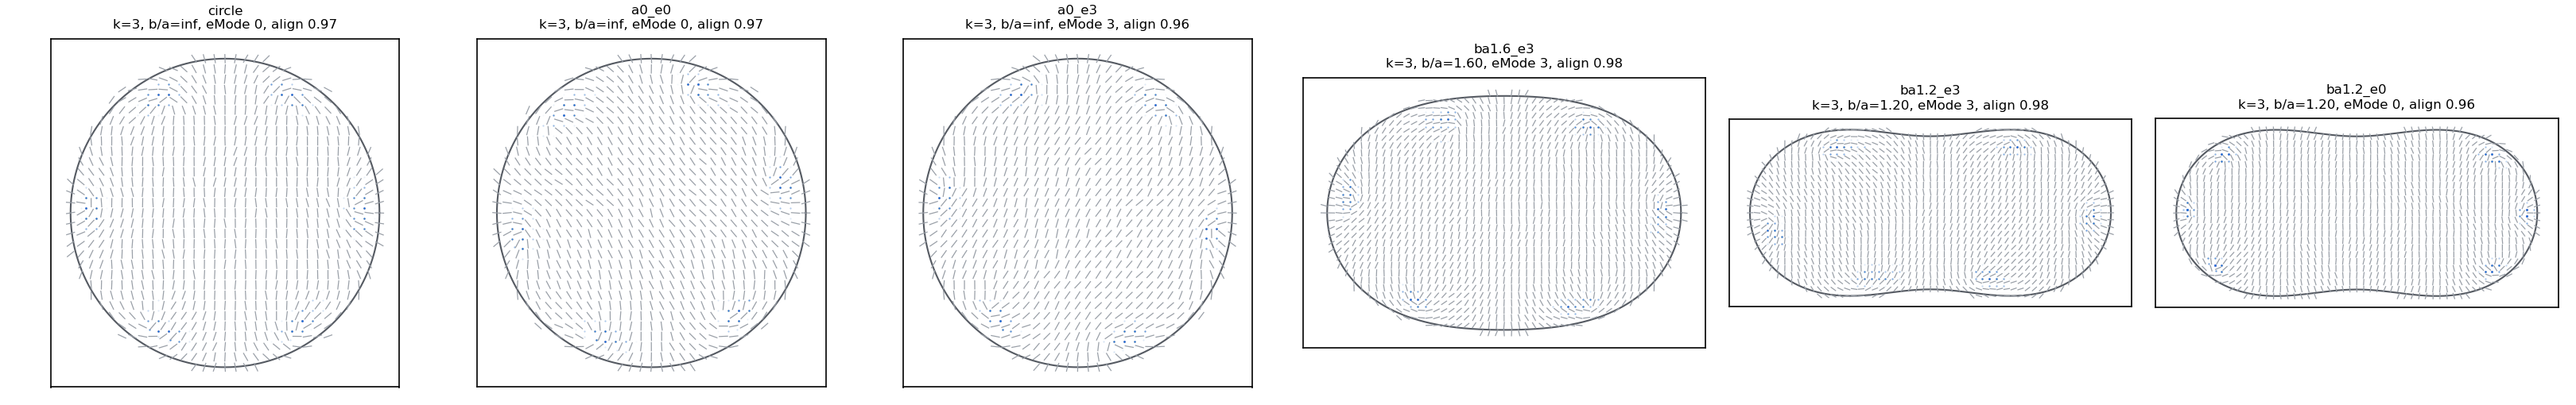
\includegraphics[width=\textwidth]{cassini_validation.png}
\caption{Passive validation of the Cassini wall ($k=3$): circle reference, $a=0$ with eMode 0 and 3, ovals $b/a=1.6$ and 1.2
with eMode 3, and $b/a=1.2$ with eMode 0.}\label{fig:cassval}
\end{figure}
\paragraph{Active length.} \SIcand
\begin{figure}[H]\centering
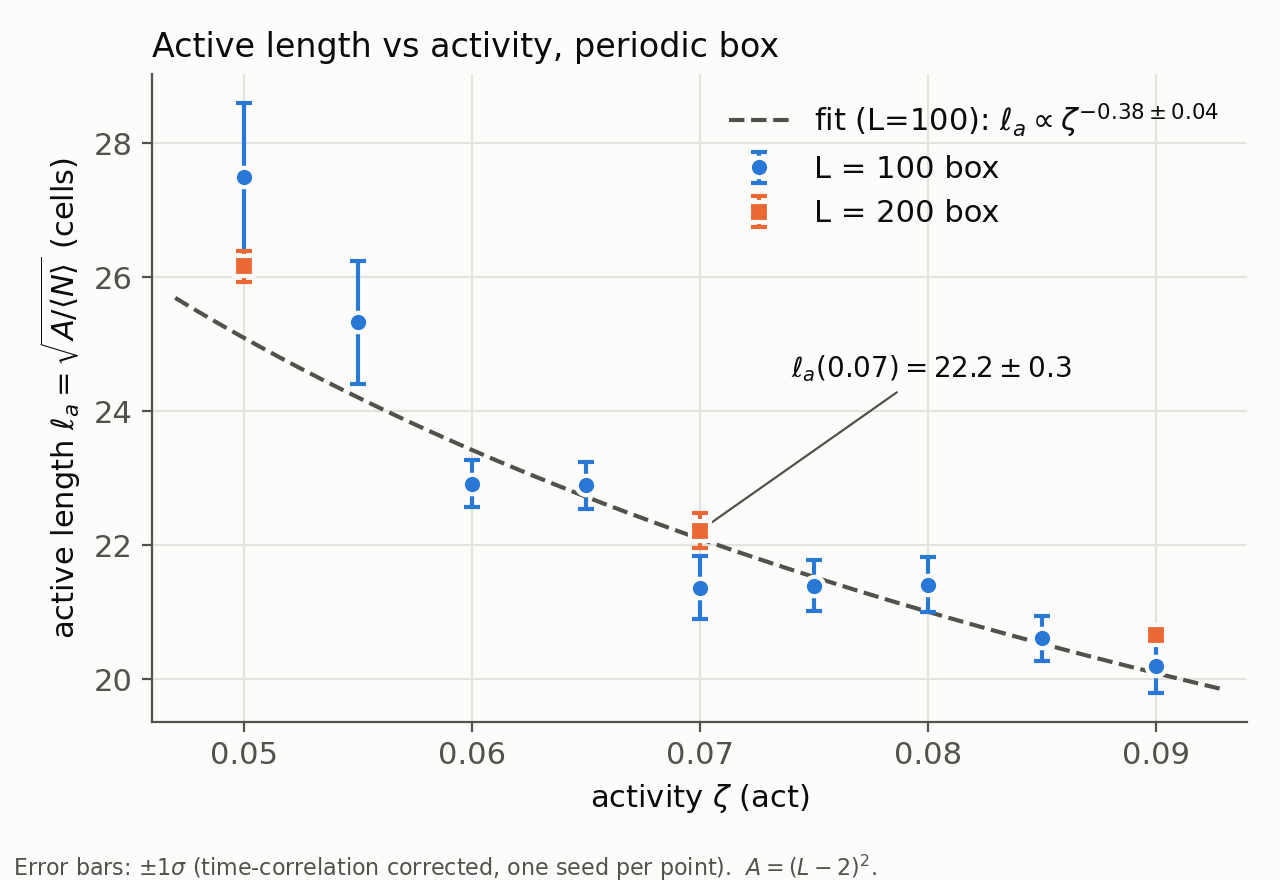
\includegraphics[width=0.75\textwidth]{active_length.png}
\caption{Active length against activity in periodic boxes of $100^2$ and $200^2$ cells, with a power-law fit.}\label{fig:la}
\end{figure}
\begin{table}[H]\centering\small
\caption{Active length (cells). $200^2$ values at 0.06 and 0.11: mean of two seeds (seed spread 1.2--1.5$\sigma$).}\label{tab:la}
\begin{adjustbox}{max width=\textwidth}
\begin{tabular}{lccccc}\toprule
$\zeta$ & 0.05 & 0.06 & 0.07 & 0.09 & 0.11\\\midrule
$\la$, $100^2$ & $27.5\pm1.1$ & $22.9\pm0.4$ & $21.4\pm0.5$ & $20.2\pm0.4$ & --\\
$\la$, $200^2$ & $26.2\pm0.2$ & $24.3\pm0.1$ & $\mathbf{22.2\pm0.3}$ & $20.7\pm0.1$ & $19.1\pm0.1$\\\bottomrule
\end{tabular}
\end{adjustbox}
\end{table}
No significant finite-size effect between the boxes (differences $-4.8\%$, $+4.0\%$, $+2.3\%$ at 0.05, 0.07, 0.09; 1.1--1.6$\sigma$).
$\la\propto\zeta^{-1/2}$ up to $\zeta\approx0.08$ ($\alpha=0.485\pm0.031$), flattening above (full range $\alpha=0.39$).
The exponent is not part of the paper (it is covered by published work); only $\la(0.07)$ enters, as the length unit.
\paragraph{Compressibility.} Density standard deviation 6.1 $\to$ 9.8 (Poisson 4.47) and rms Mach number 0.66 $\to$ 1.0
($c_s=1$) from $\zeta=0.05$ to 0.09 in periodic boxes; no threshold. In cavities the vortex adds a radial stratification
(Sec.~\ref{sec:activity}).
